\documentclass[a4paper,12pt]{article}

\usepackage[T2A]{fontenc}			
\usepackage[utf8]{inputenc}			
\usepackage[english,russian]{babel}	

\usepackage[
bookmarks=true, colorlinks=true, unicode=true,
urlcolor=black,linkcolor=black, anchorcolor=black,
citecolor=black, menucolor=black, filecolor=black,
]{hyperref}

\usepackage{color}
\usepackage{caption}
\DeclareCaptionFont{white}{\color{black}}
\DeclareCaptionFormat{listing}{\colorbox{white}{\parbox{\textwidth}{#1#2#3}}}
\captionsetup[lstlisting]{format=listing,labelfont=white,textfont=white}

\usepackage{amsmath,amsfonts,amssymb,amsthm,mathtools} 
\usepackage{wasysym}

\usepackage{graphicx}
%\usepackage[cache=false]{minted}
\usepackage{cmap}
\usepackage{indentfirst}

\usepackage{listings} 
\usepackage{fancyvrb}

\usepackage{geometry}
\geometry{left=2cm}
\geometry{right=1.5cm}
\geometry{top=1cm}
\geometry{bottom=2cm}

\setlength{\parindent}{5ex}
\setlength{\parskip}{0.5em}

\usepackage{pgfplots}
\usetikzlibrary{datavisualization}
\usetikzlibrary{datavisualization.formats.functions}

\begin{document}
	\lstset{ %
		language=C,                 % выбор языка для подсветки (здесь это С)
		basicstyle=\small\sffamily, % размер и начертание шрифта для подсветки кода
		numbers=left,               % где поставить нумерацию строк (слева\справа)
		numberstyle=\tiny,           % размер шрифта для номеров строк
		stepnumber=1,                   % размер шага между двумя номерами строк
		numbersep=5pt,                % как далеко отстоят номера строк от подсвечиваемого кода
		backgroundcolor=\color{white}, % цвет фона подсветки - используем \usepackage{color}
		showspaces=false,            % показывать или нет пробелы специальными отступами
		showstringspaces=false,      % показывать или нет пробелы в строках
		showtabs=false,             % показывать или нет табуляцию в строках
		frame=single,              % рисовать рамку вокруг кода
		tabsize=2,                 % размер табуляции по умолчанию равен 2 пробелам
		captionpos=t,              % позиция заголовка вверху [t] или внизу [b] 
		breaklines=true,           % автоматически переносить строки (да\нет)
		breakatwhitespace=false, % переносить строки только если есть пробел
		escapeinside={\%*}{*)}   % если нужно добавить комментарии в коде
	}
	
	% Титульный лист
	\begin{figure}[h!]
		\begin{center}
			{\includegraphics[scale = 0.4]{titul.jpg}}
			\label{titul}
		\end{center}
	\end{figure}
	
	\vspace*{15mm} 
	
	\huge
	\begin{center}
		Дисциплина: <<Функциональное и логическое программирование>>
	\end{center}
	\vspace*{15mm} 	
	
	\begin{center}
		Лабораторная работа №2
	\end{center}
	
	\vspace*{15mm} 	
	
	\large
	\begin{flushright}
		Студент: Левушкин И. К. \\
		Группа: ИУ7-62Б \\
		Преподаватели: Толпинская Н. Б., \\ Строганов Ю. В. \\
	\end{flushright}
	
	\vspace*{30mm}
	\begin{center}
		Москва, 2020 г.  
	\end{center}
	\thispagestyle{empty}
	
	
	\newpage
	
	\section*{3. Результат вычисления выражений (CAR, CDR)}
	
	\begin{table} [h!]
		\begin{center}
			\begin{tabular}{|l|l|}
				\hline
				{\bf  Выражение} &    {\bf Результат} \\
				\hline
				{ (caadr '((blue cube) (red pyramid)))}& RED\\
				\hline
				{(cdar '((abc) (def) (ghi)))}& NIL\\
				\hline
				{ (cadr '((abc) (def) (ghi)))}& (DEF)\\
				\hline
				{ caddr '((abc) (def) (ghi)))}& (GHI)\\
				\hline
			\end{tabular}  
			\label{m1}
		\end{center}
	\end{table}
	
	\section*{4. Результат вычисления выражений (list, cons)}
	
	\begin{table} [h!]
		\begin{center}
			\begin{tabular}{|l|l|}
				\hline
				{\bf  Выражение} &    {\bf Результат} \\
				\hline
				{ (list 'Fred 'and Wilma)}& Ошибка (variable WILMA has no value)\\
				\hline
				{(list 'Fred '(and Wilma))}& (FRED (AND WILMA))\\
				\hline
				{(cons Nil Nil)}& (NIL)\\
				\hline
				{(cons T Nil)}& (T)\\
				\hline
				{(cons Nil T)}& (NIL . T)\\
				\hline
				{(list Nil)}& (NIL)\\
				\hline
				{(cons (T) Nil)}& Ошибка (функция T не определена)\\
				\hline
				{(list '(one two) '(free temp))}& ((ONE TWO) (FREE TEMP))\\
				\hline
				{(cons 'Fred '(and Wilma))}& (FRED AND WILMA)\\
				\hline
				{(cons 'Fred '(Wilma))}& (FRED WILMA)\\
				\hline
				{(list Nil Nil)}& (NIL NIL)\\
				\hline
				{(list T Nil)}& (T Nil)\\
				\hline
				{(list Nil T)}& (Nil T)\\
				\hline
				{(cons T (list Nil))}& (T NIL)\\
				\hline
				{(list (T) Nil)}& Ошибка (функция T не определена)\\
				\hline
				{(cons '(one two) '(free temp))}& ((one two) free temp)\\
				\hline
			\end{tabular}  
			\label{m2}
		\end{center}
	\end{table}

\newpage
	
	\section*{5. Написание функций}
	
	\subsection*{ 1) (f1 ar1 ar2 ar3 ar4) возвращает список ((ar1 ar2) (ar3 ar4)): (defun f1(ar1 ar2 ar3 ar4) (list (list ar1 ar2) (list ar3 ar4)))}
	
	\begin{table} [h!]
		\begin{center}
			\begin{tabular}{|l|l|}
				\hline
				{\bf  Выражение} &    {\bf Результат} \\
				\hline
				{ (f1 1)}& Ошибка (мало аргументов)\\
				\hline
				{(f1 1 2 3 4 5)}& Ошибка (много аргументов)\\
				\hline
				{(f1 1 2 3 4)}& ((1 2) (3 4))\\
				\hline
				{(f1 'a 'b 'c 'd)}& ((A B) (C D))\\
				\hline
				{(f1 T Nil 'a 4)}& ((T NIL) (A 4))\\
				\hline
				{(f1 1 '(2 z) 3 4)}& ((1 (2 Z)) (3 4))\\
				\hline
			\end{tabular}  
			\label{m3}
		\end{center}
	\end{table}

	\begin{figure}[h!]
		\begin{center}
			{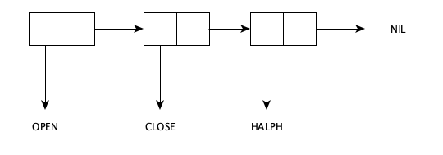
\includegraphics[scale = 0.4]{first.jpg}}
			\label{first}
		\end{center}
	\end{figure}
	
	\subsection*{ 2) (f2 ar1 ar2) возвращает список ((ar1) (ar2)): (defun f2(ar1 ar2) (list (list ar1) (list ar2)))}
	
	\begin{table} [h!]
		\begin{center}
			\begin{tabular}{|l|l|}
				\hline
				{\bf  Выражение} &    {\bf Результат} \\
				\hline
				{ (f2 1)}& Ошибка (мало аргументов)\\
				\hline
				{(f2 1 2 3 4 5)}& Ошибка (много аргументов)\\
				\hline
				{(f2 1 2)}& ((1) (2))\\
				\hline
				{(f2 'a 'b)}& ((A B) (C D))\\
				\hline
				{(f2 T Nil)}& ((T) (NIL))\\
				\hline
				{(f2 '(a b c) '((u v)))}& (((A B C)) (((U V))))\\
				\hline
			\end{tabular}  
			\label{m4}
		\end{center}
	\end{table}

	\begin{figure}[h!]
		\begin{center}
			{\includegraphics[scale = 0.4]{second.jpg}}
			\label{second}
		\end{center}
	\end{figure}
	
	\subsection*{ 3) (f3 ar1) возвращает список (((ar1))): (defun f3(ar1) (list (list (list ar1))))}
	
	\begin{table} [h!]
		\begin{center}
			\begin{tabular}{|l|l|}
				\hline
				{\bf  Выражение} &    {\bf Результат} \\
				\hline
				{ (f3)}& Ошибка (мало аргументов)\\
				\hline
				{(f3 1 2 3 4 5)}& Ошибка (много аргументов)\\
				\hline
				{(f3 1)}& (((1)))\\
				\hline
				{(f3 'a)}& (((A B)))\\
				\hline
				{(f3 '((1 2) (D T)))}& (((((1 2) (D T)))))\\
				\hline
			\end{tabular}  
			\label{m5}
		\end{center}
	\end{table}

	\begin{figure}[h!]
		\begin{center}
			{\includegraphics[scale = 0.4]{third.jpg}}
			\label{third}
		\end{center}
	\end{figure}
	
	\section*{Классификация функций}
	
	\begin{enumerate}
		\item Чистые функции (фиксированное число аргументов и единственный результат)
		\item Формы (переменное число аргументов или аргументы обрабатываются поразному)
		Функционалы (в качестве аргумента передается функция)
	\end{enumerate}

\section*{Классификация базовых функций}

\begin{enumerate}
	\item Селекторы
	\item Конструкторы
	\item Предикаты
\end{enumerate}

	
\end{document}